\documentclass[10pt]{beamer}
\usetheme[
%%% option passed to the outer theme
%    progressstyle=fixedCircCnt,   % fixedCircCnt, movingCircCnt (moving is deault)
  ]{Feather}
  
% If you want to change the colors of the various elements in the theme, edit and uncomment the following lines

% Change the bar colors:
%\setbeamercolor{Feather}{fg=red!20,bg=red}

% Change the color of the structural elements:
%\setbeamercolor{structure}{fg=red}

% Change the frame title text color:
%\setbeamercolor{frametitle}{fg=blue}

% Change the normal text color background:
%\setbeamercolor{normal text}{fg=black,bg=gray!10}

%-------------------------------------------------------
% INCLUDE PACKAGES
%-------------------------------------------------------

\usepackage[utf8]{inputenc}
\usepackage[english]{babel}
\usepackage[T1]{fontenc}
\usepackage{graphicx}
\usepackage{helvet}

%-------------------------------------------------------
% DEFFINING AND REDEFINING COMMANDS
%-------------------------------------------------------

% colored hyperlinks
\newcommand{\chref}[2]{
  \href{#1}{{\usebeamercolor[bg]{Feather}#2}}
}

%-------------------------------------------------------
% INFORMATION IN THE TITLE PAGE
%-------------------------------------------------------

\title[] % [] is optional - is placed on the bottom of the sidebar on every slide
{ % is placed on the title page
      \textbf{CI/CD}
}

\subtitle[Descomplicando o CI/CD]
{
      \textbf{CI/CD}
}

\author[Eugenio Cunha]
{      Eugenio Cunha
      {}
}

\institute[]
{
      TWT Info
  %there must be an empty line above this line - otherwise some unwanted space is added between the university and the country (I do not know why;( )
}

\date{\today}

%-------------------------------------------------------
% THE BODY OF THE PRESENTATION
%-------------------------------------------------------

\begin{document}

%-------------------------------------------------------
% THE TITLEPAGE
%-------------------------------------------------------

% {\1% % this is the name of the PDF file for the background



\begin{frame}{Descomplicando o CI/CD}{}
    \begin{center}
        
\includegraphics[scale=0.3]{images/cicd}
    \end{center}
\end{frame}

\section{Content}

%-------------------------------------------------------
\subsection{Descomplicando o CI/CD}
\begin{frame}{Conteúdo}{Descomplicando o CI/CD}
  \begin{itemize}
    \item O que é CI/CD?
    \item CI/CD é um Hype da tecnologia?
    \item CI/CD é parte da cultura DevOps?
    \item Talk is cheap. Show me the code.
  \end{itemize}
\end{frame}
%-------------------------------------------------------

%-------------------------------------------------------
\section{Introduction}
\subsection{Descomplicando o CI/CD}
\begin{frame}{O que é CI/CD?}{Descomplicando o CI/CD}
  \begin{center}
    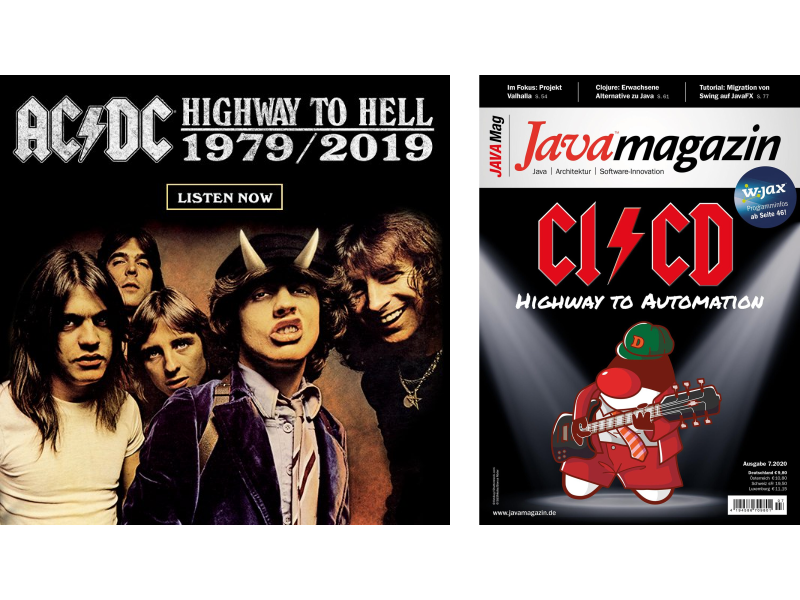
\includegraphics[scale=0.38]{images/acdc.png}
  \end{center}
   \begin{center}
      Não é uma banda de rock'n'roll! Eles são AC/DC.
   \end{center}
\end{frame}
%-------------------------------------------------------

%-------------------------------------------------------
\section{Introduction}
\subsection{Descomplicando o CI/CD}
\begin{frame}{O que é CI/CD?}{Descomplicando o CI/CD}
    \begin{center}
      ``CI ou Integração Contínua, é uma prática de desenvolvimento de software na qual você compila e testa software toda vez que um desenvolvedor envia código para o repositório, e isso acontece várias vezes ao dia.''
      
      ``CD ou Entrega Contínua é uma abordagem de engenharia de software na qual a integração contínua, testes automatizados e recursos de implantação automatizada permitem que o software seja desenvolvido e implementado de forma rápida, confiável e repetitiva com intervenção humana mínima''
    \end{center}
\end{frame}
%-------------------------------------------------------

%-------------------------------------------------------
\section{CICD}
\subsection{Descomplicando o CI/CD}
\begin{frame}{O que é CI?}{Descomplicando o CI/CD}
  \begin{center}
    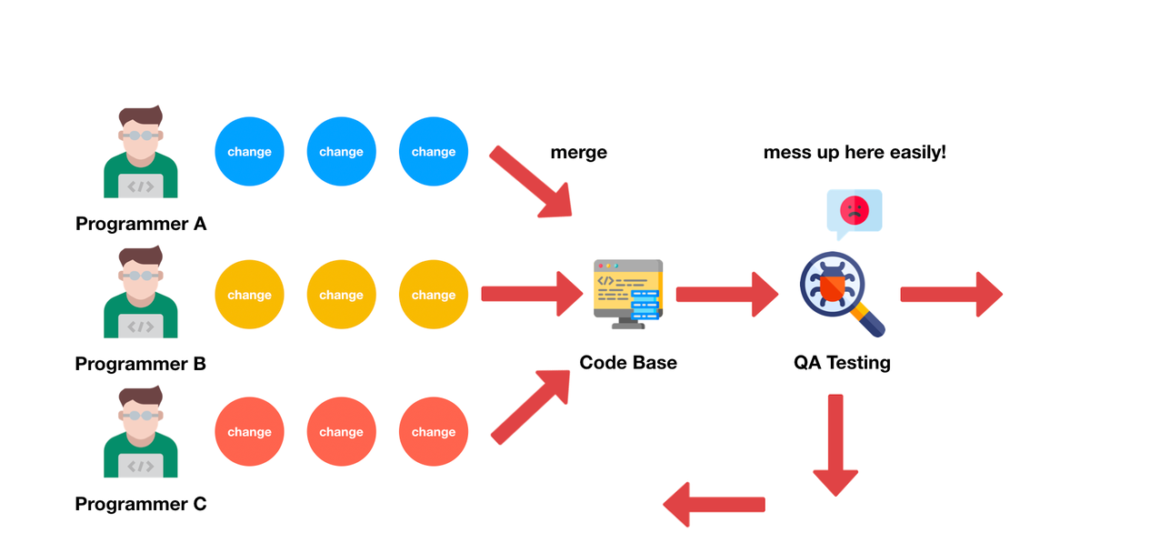
\includegraphics[scale=0.25]{images/traditional.png}
  \end{center}
  \begin{center}
      Desenvolvimento de software tradicional.
   \end{center}
\end{frame}
%-------------------------------------------------------

%-------------------------------------------------------
\section{CICD}
\subsection{Descomplicando o CI/CD}
\begin{frame}{O que é CI/CD?}{Descomplicando o CI/CD}
  \begin{center}
    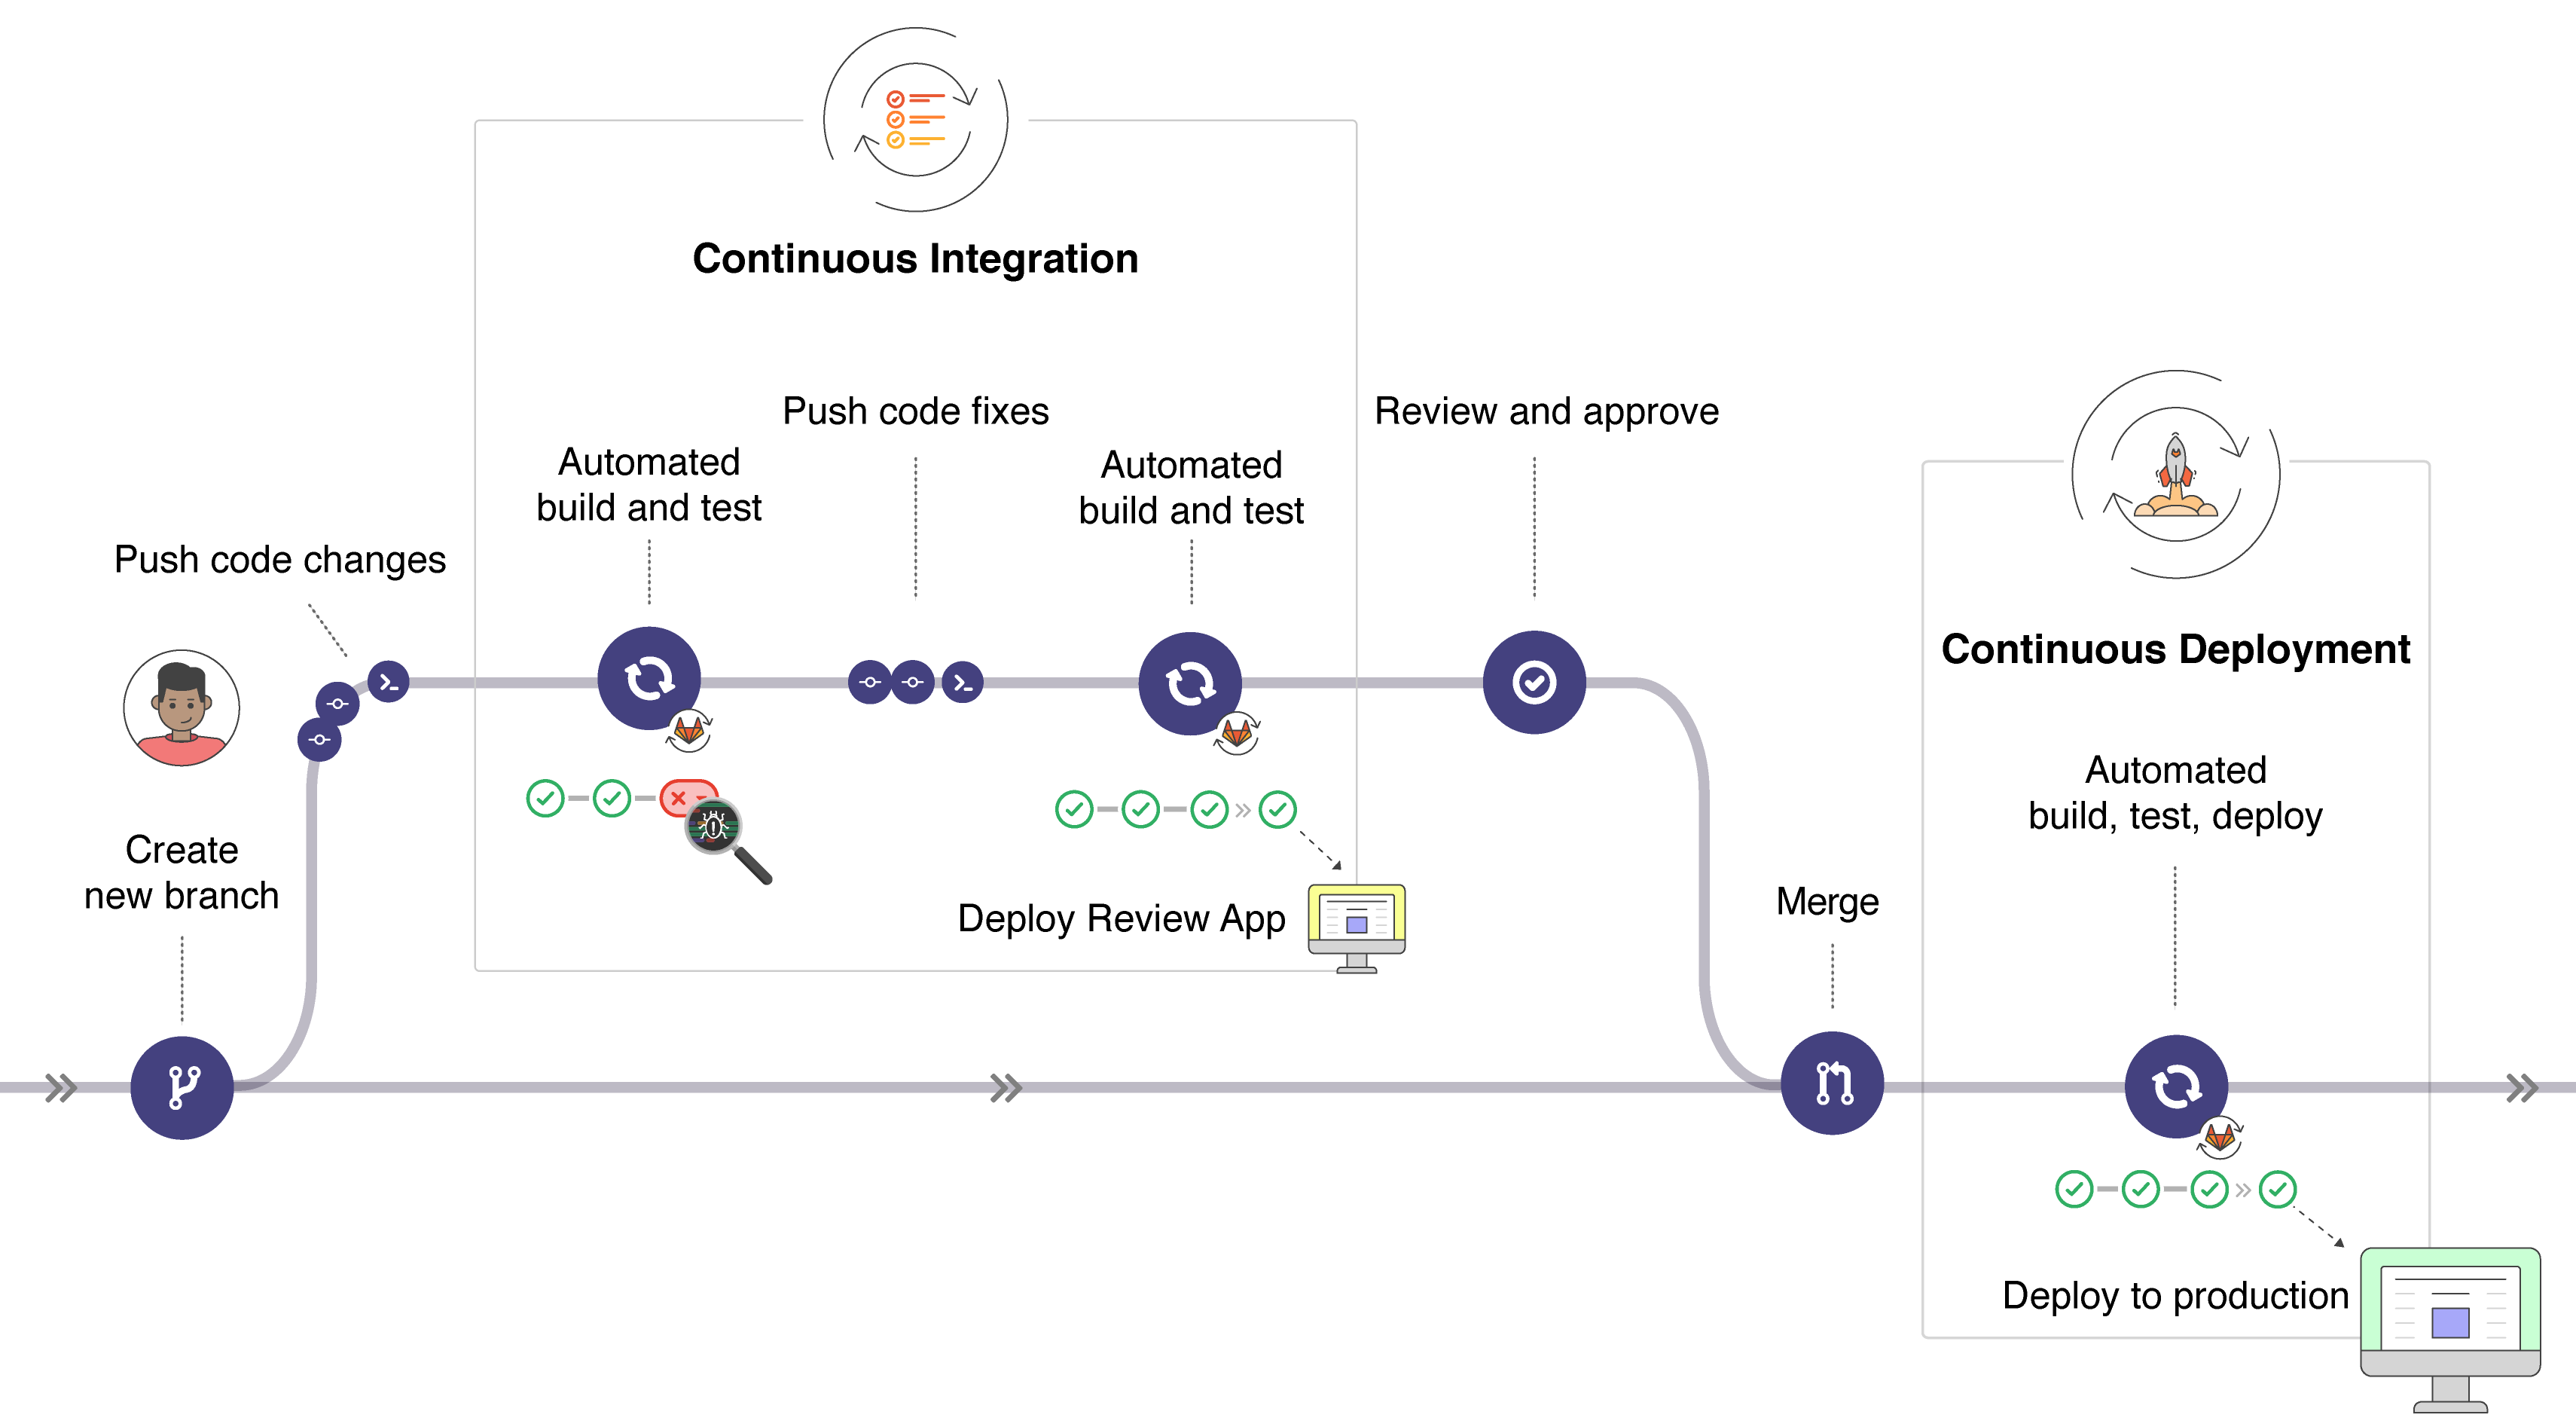
\includegraphics[scale=0.09]{images/workflow.png}
  \end{center}
  \begin{center}
      Desenvolvimento de software com CI\textbackslash CD.
   \end{center}
\end{frame}
%-------------------------------------------------------

%-------------------------------------------------------
\section{HYPE}
\subsection{Descomplicando o CI/CD}
\begin{frame}{CI/CD um Hype da tecnologia?}{Descomplicando o CI/CD}
    \begin{center}
     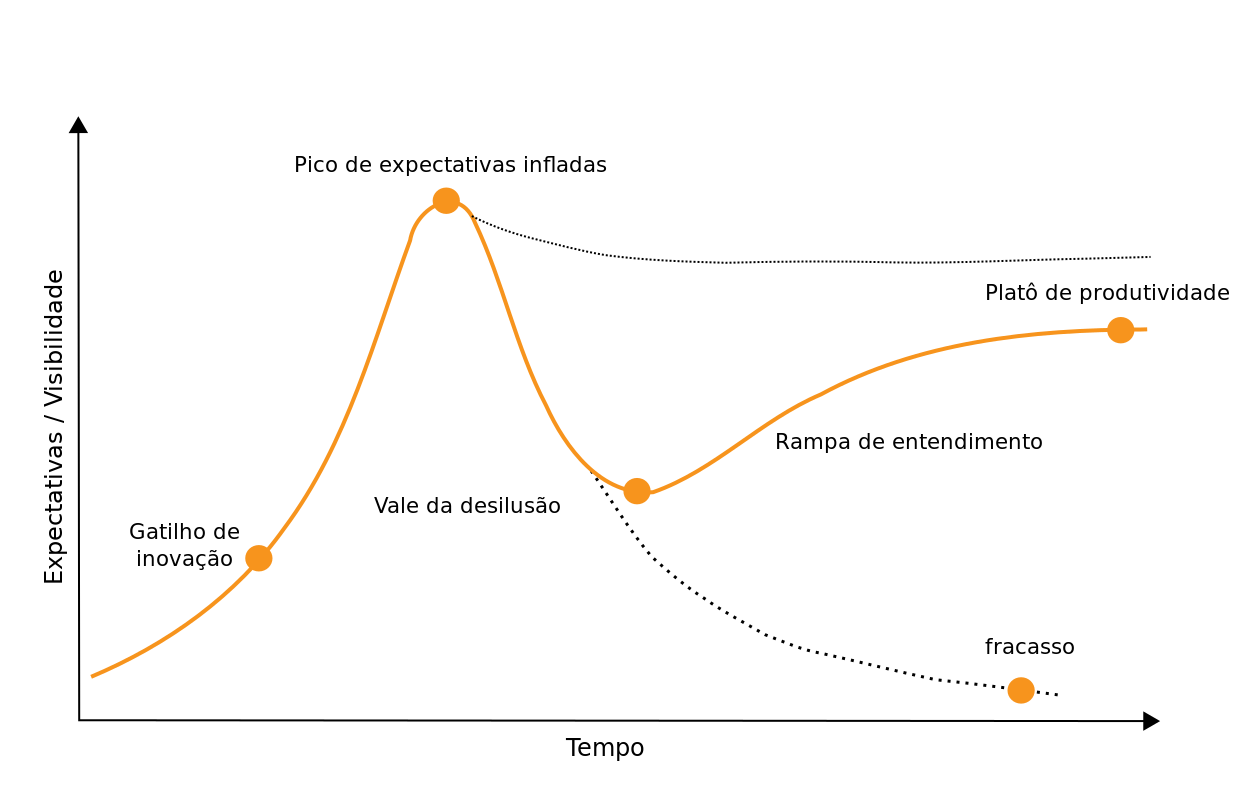
\includegraphics[scale=0.25]{images/hype.png}
    \end{center}
\end{frame}
%-------------------------------------------------------

%-------------------------------------------------------
\section{DEVOPS}
\subsection{Descomplicando o CI/CD}
\begin{frame}{CI/CD é parte da cultura DevOps?}{Descomplicando o CI/CD}
    \begin{center}
     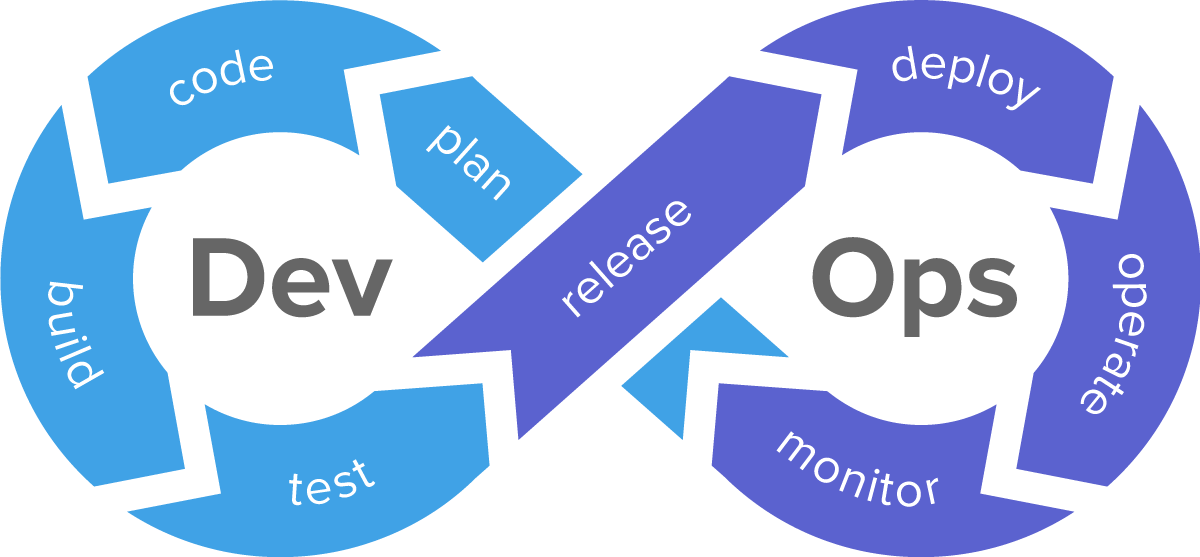
\includegraphics[scale=0.25]{images/devops}
    \end{center}
\end{frame}
%-------------------------------------------------------

%-------------------------------------------------------
\section{Tools}
\subsection{Descomplicando o CI/CD}
\begin{frame}{Ferramentas CI/CD}{Descomplicando o CI/CD}
    \begin{itemize}
     \item www.gitlab.com
     \item www.github.com
     \item www.jenkins.io
    \end{itemize}
\end{frame}
%-------------------------------------------------------

\section{Installation}
%-------------------------------------------------------
\subsection{Source files}
\begin{frame}{Installation}{Source files}
%-------------------------------------------------------

\begin{block}{}
The theme contains 4 source files:
  \begin{itemize}
    \item {\tt beamercolorthemeFeather.sty}
    \item {\tt beamerouterthemeFeather.sty}
    \item {\tt beamerinnerthemeFeather.sty}
    \item {\tt beamerthemeFeather.sty}
  \end{itemize}
\end{block}
\end{frame}

%-------------------------------------------------------
\subsection{Local and Global installation}
\begin{frame}{Installation}{Local and Global installation}
%-------------------------------------------------------
  The theme can be installed for \textbf{local} or \textbf{global} use.
  \pause
  \begin{block}{Local Installation}
  \begin{itemize}    
    \item Local installation is the simplest way of installing the theme. 
    \item You need to placing the 4 source files in the same folder as your presentation. When you download the theme, the 4 theme files are located in the {\tt local} folder.
  \end{itemize}
  \end{block}

  \begin{block}{Global Installation}
  \begin{itemize}
     \item If you wish to make the theme globally available, you must put the files in your local latex directory tree. The location of the root of the local directory tree depends on your operating system and the latex distribution. 
     \item Detailed steps on how to proceed installation under various operating systems can be found at Beamer documentation.
  \end{itemize}
  \end{block}
\end{frame}
     

%-------------------------------------------------------
\subsection{Required Packages}
\begin{frame}{Installation}{Required Packages}
%-------------------------------------------------------

  For using the Feather Theme you will need the Bemaer class installed and the following 2 packages
  \begin{itemize}
    \item TikZ\footnote{TikZ is a package for creating beautiful graphics. Have a look at these \chref{http://www.texample.net/tikz/examples/}{online examples} or the \chref{http://tug.ctan.org/tex-archive/graphics/pgf/base/doc/generic/pgf/pgfmanual.pdf}{pgf user manual}.}
    \item calc
  \end{itemize}
  Due to the fact that the packages are very common they should be included in your latex distribution in the first place.
\end{frame}

%-------------------------------------------------------
\section{User Interface}
\subsection{Loading the Theme and Theme Options}
\begin{frame}{User Interface}{Loading the Theme and Theme Options}
%-------------------------------------------------------

  \begin{block}{The Presentation Theme}
    The Feather Theme can be loaded in a familiar way. In the reamble of your {\tt tex} file you must type\\ \vspace{5pt} 
    {\tt \textbackslash usetheme[<options>]\{Feather\}}\\ \vspace{5pt} 
    The presentation theme loads the inner, outer and color Feather theme files and passes the {\tt <options>} on to these files.
  \end{block}
  \begin{block}{The Inner and Outher Themes}
    If you wish you can load only the inner, or the outher theme directly by\\ \vspace{5pt} 
    {\tt \textbackslash useinnertheme\{Feather\}} (and it has no options)\\ \vspace{5pt} 
    {\tt \textbackslash useoutertheme[<options>]\{Feather\}} (it has one option)\\
    \hspace{20pt}{\tt progressstyle=\{fixedCircCnt or movingCircCnt\}} \\
    \begin{itemize}
    \item which set how the progress is illustrated;
    \item the value {\tt movingCircCnt} is the default.
    \end{itemize}
  \end{block}
\end{frame}

\begin{frame}{User Interface}{Loading the Theme and Theme Options}

  \begin{block}{The Color Theme}
    Also you can load only the color theme by writing in the preamble of the {\tt tex} file 
    
    \vspace{5pt} 
    
    \begin{itemize}
    \item {\tt \textbackslash usecolortheme\{Feather\}}
    \end{itemize}
    
    \vspace{5pt}
    
    ...or to change the colors of the various elements in the theme
    
    \vspace{5pt} 
    \begin{itemize}
    \item Change the bar colors: \\    
    {\tt \textbackslash setbeamercolor \{Feather\}\{fg=<color>, bg=<color>\}}
    
    \vspace{2pt} 
    
    \item Change the color of the structural elements: \\    
    {\tt \textbackslash setbeamercolor\{structure\}\{fg=<color>\}}
    
    \vspace{2pt} 
    
    \item Change the frame title text color:\\
    {\tt \textbackslash setbeamercolor\{frametitle\}\{fg=<color>\}}
    
    \vspace{2pt} 
    
    \item Change the normal text color background:    
    {\tt \textbackslash setbeamercolor\{normal text\}\{fg=<color>, bg=<color>\}}
    \end{itemize}
  \end{block}
\end{frame}


%-------------------------------------------------------
\subsection{Feather image}
\begin{frame}{User Interface}{The Feather Background Image}
%-------------------------------------------------------

\begin{block}{The Feather Background Image}
    \begin{itemize}
    \item In Feather theme, the title page frame and the last frame have the Feather image as the background image. 
    \item The Feather background image can be produced to any frame by wrating on the begining at the choosen frame the following
    \end{itemize} 
    
    \vspace{5pt} 
    
  {\tt \{\textbackslash 1bg\\
    \textbackslash begin\{frame\}[<options>]\{Frame Title\}\{Frame Subtitle\}\\
    \ldots\\
    \textbackslash end\{frame\}\}}
\end{block}
\end{frame}


{\1
\begin{frame}[plain,noframenumbering]
  \finalpage{Thank you for using Feather Beamer Theme!}
\end{frame}}

\end{document}